\documentclass[12pt, letterpaper, titlepage]{article}

\usepackage{graphicx}
\usepackage{hyperref}

\author{Saba Saba}
\title{\textbf{TSK Typer} \\
\hrulefill \\
Finger Positioning Rules}

\begin{document}
\maketitle

\tableofcontents
\newpage
\listoffigures
\newpage

\section{Finger Positions}
\begin{figure}[h]
\centering
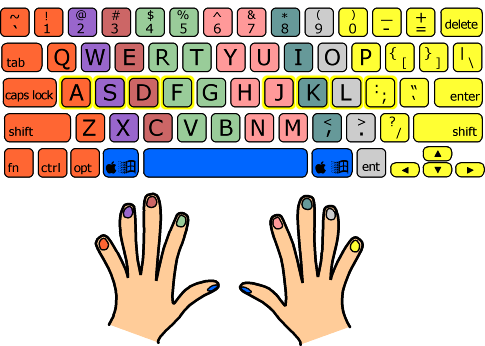
\includegraphics[width=0.5\textwidth]{which_fingers.png}
\caption{Finger-to-key mapping~\cite{hudson.misc}}
\label{Mapping}
\end{figure}
When the user is not typing, each finger must rest on the home row.
Due to the structure of the hand, the finger-to-key mapping described in figure~\ref{Mapping} is used.
This mapping illustrates how each finger generally moves in a vertical fashion along the keyboard.
The main exceptions are the pinkies, the index fingers and the thumbs:
pinkies are used to reach keys on the outer ends of the keyboard, the index fingers are used for the middle of the keyboard and the thumbs focus on the bottom of the keyboard.

\subsection{Simplified Typing}
Assume that a user begins in the resting position.
The user presses a single key before returning to the resting position.
This results in a simple validation algorithm for determining correct positioning:
\begin{enumerate}
\item Map pressed key to a finger according to figure~\ref{Mapping}
\item Ensure that each finger not equal to the above finger is resting on a home row key
\end{enumerate}

\subsection{Fast Typing}


\bibliographystyle{ieeetr}
\clearpage
\phantomsection
\addcontentsline{toc}{section}{\textbf{References}}
\bibliography{report}
\end{document}
